
%
% 
% Module: carrier_recovery_theory_tutorial
%
% Author: Michael Kramer
%
%

The phase locked loop is a critical component in coherent communications
receivers that is responsible for locking onto the carrier of a received 
modulated signal.  
Ideally the transmitted carrier frequency is known and we need
to know its phase for accurate demodulation.  However, due
to imperfections at the transmitter, the actual carrier frequency
may be slightly different than the expected frequency.  For example, in the 
QPSK transmitter of Lab 5 if the digital carrier frequency is $\frac{\pi}{2}$
and the D/A is operating at 44.1 kHz, then the expected analog carrier 
frequency is $f_c = \frac{\frac{\pi}{2}}{2 \pi} * 44.1 \: kHz \: = 11.025 kHz$.
If there is a slight change to the D/A sample rate 
(say $F_s = 44.05 kHz$) then there will be a corresponding 
change in the actual analog carrier frequency ($f_c = 11.0125 \: kHz$).

This difference between the expected and actual carrier frequencies
can be modeled as a time-varying phase.  
Provided that the frequency mismatch is small relative to the
carrier frequency, the feed-back control of an appropriately
calibrated PLL can track this time-varying phase, thereby locking
onto the correct frequency as well as phase.

\begin{figure}[ht]
   \begin{center}
      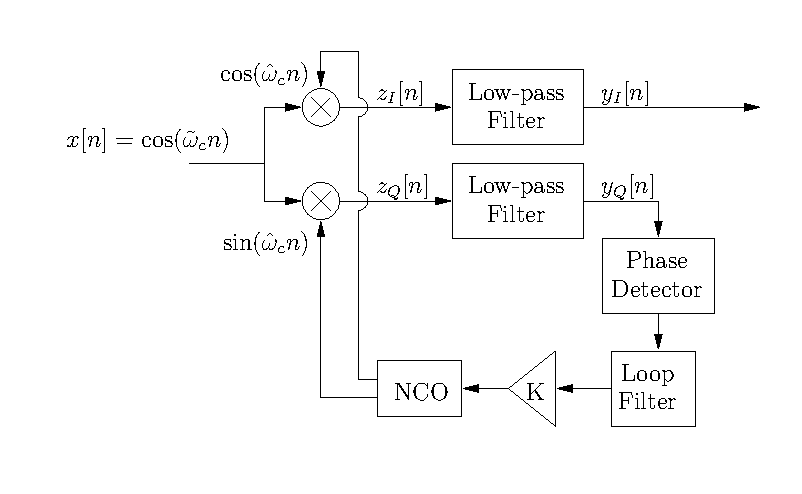
\epsfig{file=pll.eps,width=10cm}
      \caption{PLL block diagram.}
      \label{fig: PLL}
   \end{center}
\end{figure}

\paragraph{Numerically Controlled Oscillator:}

In a complete coherent receiver implementation, carrier
recovery is required since the receiver typically does not know
the exact phase and frequency of the transmitted carrier.
In an analog system this recovery is often implemented with
a voltage-controlled oscillator (VCO) that allows for precise
adjustment of the carrier frequency based on the output of
a phase detecting circuit.

In our digital application, this adjustment is performed
with a numerically controlled oscillator (NCO) (see Figure
\ref{fig: PLL}).  A simple
scheme for implementing an NCO is based on the following
re-expression of the carrier sinusoid
\bea
\sin(\lambda_c n + \theta_c) & = & \sin ( \theta(n) ) \nonumber 
\eea
where $\theta(n) = \lambda_c n + \theta_c$ ($\lambda_c$ and $\theta_c$
represent the carrier frequency and phase respectively).
This time-varying phase term can be expressed as $\theta(n) = 
\left( \sum_{m=0}^{n} \lambda_c \right) + \theta_c$ and then recursively as
\bea
\theta(n) & = & \theta(n-1) + \lambda_c
\eea
The NCO can keep track of the phase, $\theta(n)$, and force a phase offset
in the demodulating carrier by incorporating an extra term in this
recursive update
\bea
\theta(n) & = & \theta(n-1) + \lambda_c + \delta_{pd}(n)
\label{eq: phase_update}
\eea
where $\delta_{pd}(n)$ is the amount of desired phase offset
at time $n$. (What would $\delta_{pd}(n)$ look like to generate
a frequency offset?)

\paragraph{Phase Detector:}

The goal of the PLL is to maintain a demodulating sine
and cosine that match the incoming carrier frequency.
Suppose $\lambda_c$ is the believed digital
carrier frequency.  We can then represent the actual 
received carrier frequency as the expected carrier frequency
with some offset, $\tilde{\lambda}_c n = \lambda_c n + \tilde{\theta}(n)$.
The NCO generates the demodulating sine and cosine with 
the expected digital frequency $\lambda_c$ and offsets this
frequency with the output of the loop filter.  The NCO
frequency can then be modeled as $\hat{\lambda}_c n = \lambda_c n
+ \hat{\theta}(n)$.  
Using the appropriate trigonometric identities\footnote{
$\cos(A) \cos(B) = \frac{1}{2} \left[ \cos (A-B) + \cos(A+B) \right]$
and 
$\cos(A) \sin(B) = \frac{1}{2} \left[ \sin (B-A) + \sin(A+B) \right]$
}, the in-phase
and quadrature signals can be expressed as
\bea
z_I(n) & = & \frac{1}{2} \left[ \cos (\tilde{\theta}(n) - \hat{\theta}(n) )
+ \cos ( 2 \lambda_c + \tilde{\theta}(n) + \hat{\theta}(n) ) \right]
\nonumber\\
z_Q(n) & = & \frac{1}{2} \left[ \sin (\hat{\theta}(n) - \tilde{\theta}(n) )
+ \sin ( 2 \lambda_c + \tilde{\theta}(n) + \hat{\theta}(n) ) \right]
\eea
After applying a low-pass filter to remove the double frequency
terms we have
\bea
y_I(n) & = & \frac{1}{2}  \cos (\tilde{\theta}(n) - \hat{\theta}(n) )
\nonumber\\
y_Q(n) & = & \frac{1}{2}  \sin (\hat{\theta}(n) - \tilde{\theta}(n))
\eea

Note that the quadrature signal, $z_Q(n)$, is zero
when the received carrier and internally generated 
waves are exactly matched in frequency and phase.  When the phases 
are only slightly mismatched we can use the relation
\bea
\sin(\theta) \approx \theta & &\mbox{ for small } \theta \nonumber
\eea
and let the current value of the quadrature channel approximate the
phase difference: $z_Q(n) \approx (\hat{\theta}(n) - \tilde{\theta}(n))$.
With the exception of the sign error, this difference is essentially how 
much we need to offset our NCO frequency by 
(if $(\hat{\theta}(n) - \tilde{\theta}(n)) >0$
then $\hat{\theta}(n)$ is too large and we want to decrease our NCO
phase)
To make sure that the sign of the phase estimate is right,
in this example the phase detector is simply minus-one times
the value of the quadrature signal.  
In a more advanced receiver, information from both the in-phase
and quadrature branches is used to generate an estimate of
the phase error.  (What should the relationship between the I and Q
branches be for a digital QPSK signal?)

\paragraph{Loop Filter:}

The estimated phase mismatch estimate is fed to the NCO via a loop-filter,
often a simple low-pass filter. For this exercise you can use a 1-tap 
IIR filter,
\bea
y(n) & = & \beta x(n) + \alpha y(n-1)
\eea
To ensure that the DC term of the filter is at unity gain we select
$\beta = 1 - \alpha$.

It is suggested that you start by choosing $\alpha = 0.6$ and $K = 0.15$ 
for the loop-gain.  Once you have a working system, investigate
the effects of modifying these values.
